% Protocol V4 figures and tables. Needs: \usepackage{graphicx,booktabs}. Put this folder next to figures/ and tables/.

\begin{figure}[t]
\centering
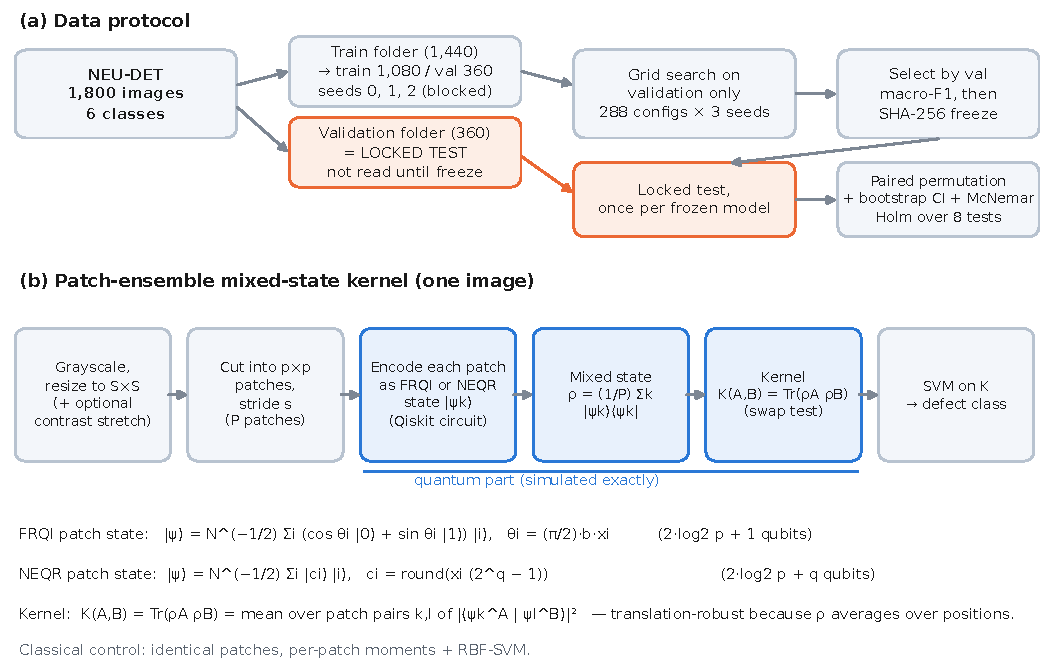
\includegraphics[width=\linewidth]{figures/Fig01_methodology_flowchart.pdf}
\caption{Methodology. (a) Data protocol: validation-only model selection, SHA-256 freeze, one locked-test evaluation per frozen model and pre-declared statistics. (b) The patch-ensemble mixed-state kernel for one image.}
\label{fig:fig01}
\end{figure}

\begin{figure}[t]
\centering
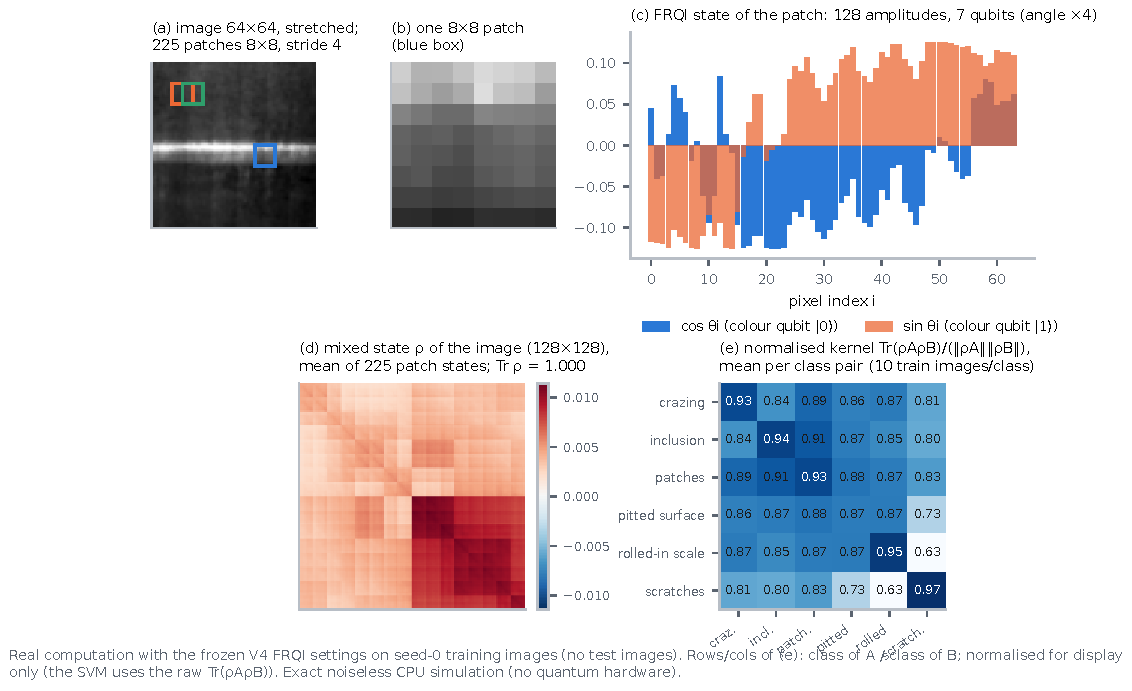
\includegraphics[width=\linewidth]{figures/Fig02_patch_encoding_illustration.pdf}
\caption{The method on a real NEU-DET training image (frozen FRQI settings: 64$\times$64, 8$\times$8 patches, stride 4). (a) image and example patches; (b) one patch; (c) its 7-qubit FRQI amplitudes; (d) the image's mixed state $\rho$; (e) normalised kernel between classes (10 training images per class).}
\label{fig:fig02}
\end{figure}

\begin{figure}[t]
\centering
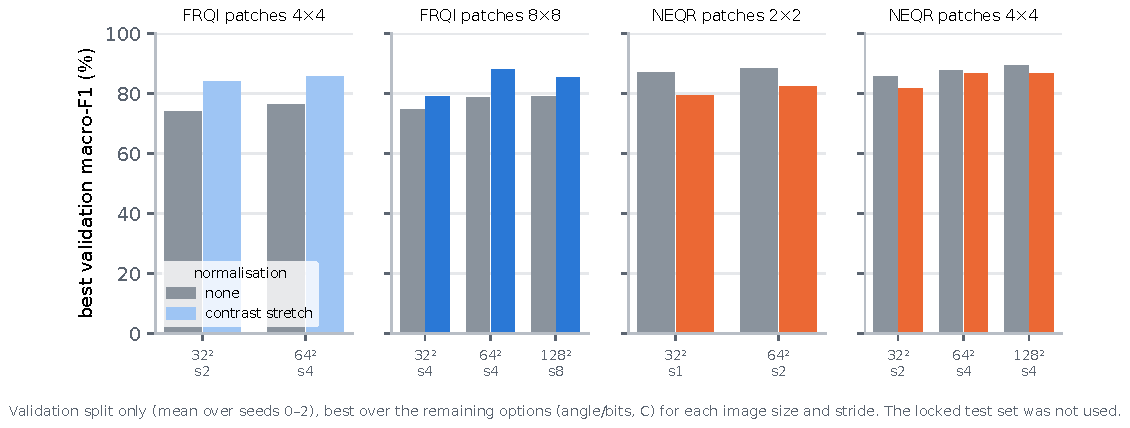
\includegraphics[width=\linewidth]{figures/Fig09_validation_sweep.pdf}
\caption{Validation-only hyper-parameter sweep: best validation macro-F1 for each image size / stride and normalisation. The locked test set was not used.}
\label{fig:fig09}
\end{figure}

\begin{figure}[t]
\centering
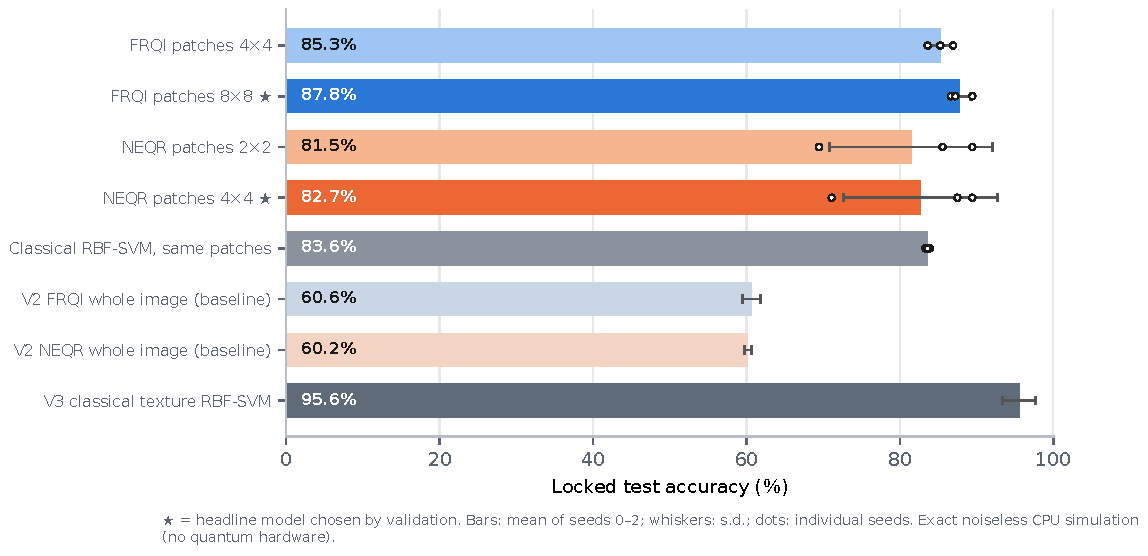
\includegraphics[width=\linewidth]{figures/Fig03_main_results.pdf}
\caption{Locked-test accuracy of all V4 groups and reference models (mean $\pm$ s.d. over seeds 0--2; dots = individual seeds; $\star$ = headline chosen by validation).}
\label{fig:fig03}
\end{figure}

\begin{figure}[t]
\centering
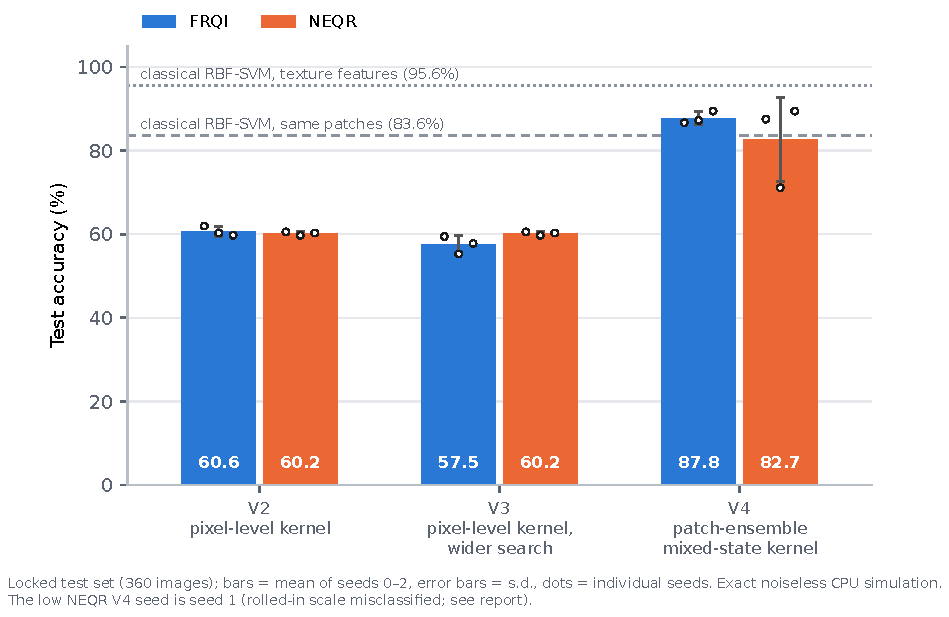
\includegraphics[width=\linewidth]{figures/Fig04_frqi_neqr_across_protocols.pdf}
\caption{FRQI and NEQR test accuracy across protocols V2, V3 and V4, with classical references.}
\label{fig:fig04}
\end{figure}

\begin{figure}[t]
\centering
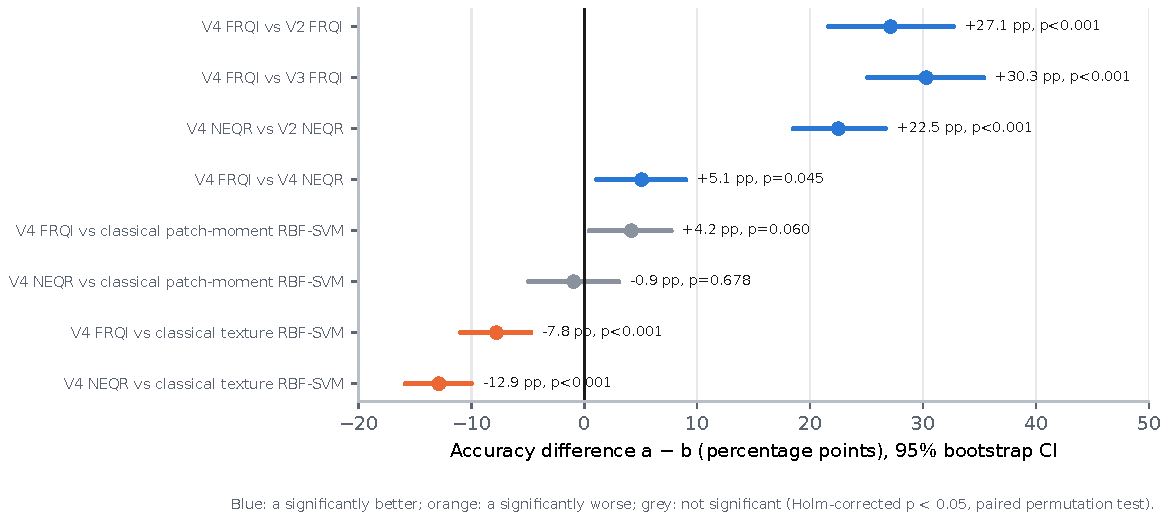
\includegraphics[width=\linewidth]{figures/Fig05_comparisons_forest.pdf}
\caption{The eight pre-declared paired comparisons: accuracy difference with 95 \% bootstrap CI and Holm-corrected p-values.}
\label{fig:fig05}
\end{figure}

\begin{figure}[t]
\centering
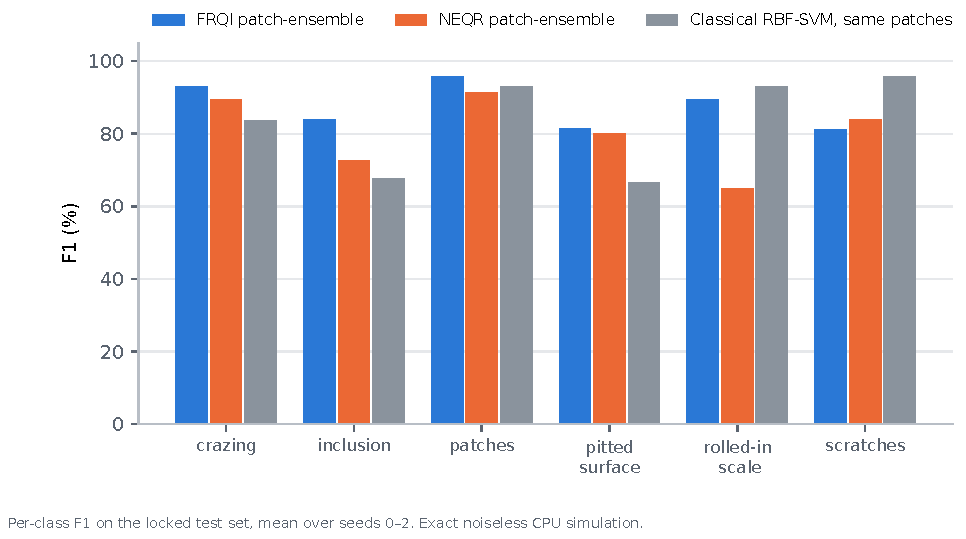
\includegraphics[width=\linewidth]{figures/Fig07_per_class_f1.pdf}
\caption{Per-class F1 on the locked test set (mean over seeds).}
\label{fig:fig07}
\end{figure}

\begin{figure}[t]
\centering
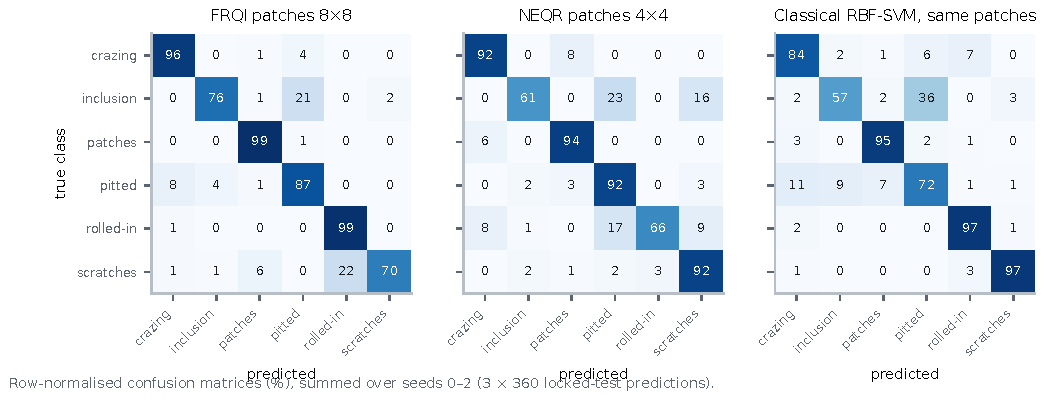
\includegraphics[width=\linewidth]{figures/Fig06_confusion_matrices.pdf}
\caption{Row-normalised confusion matrices summed over seeds 0--2.}
\label{fig:fig06}
\end{figure}

\begin{figure}[t]
\centering
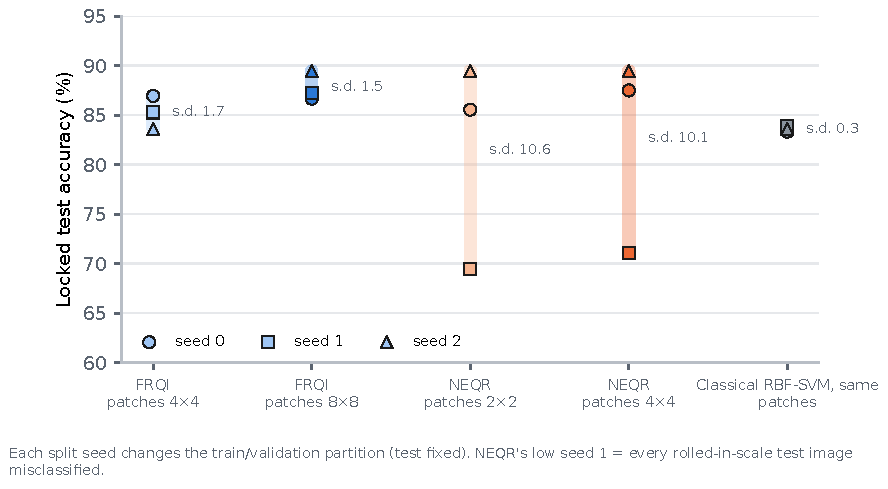
\includegraphics[width=\linewidth]{figures/Fig08_seed_stability.pdf}
\caption{Test accuracy of each split seed. NEQR's seed-1 drop is caused by the rolled-in-scale class.}
\label{fig:fig08}
\end{figure}

\begin{figure}[t]
\centering
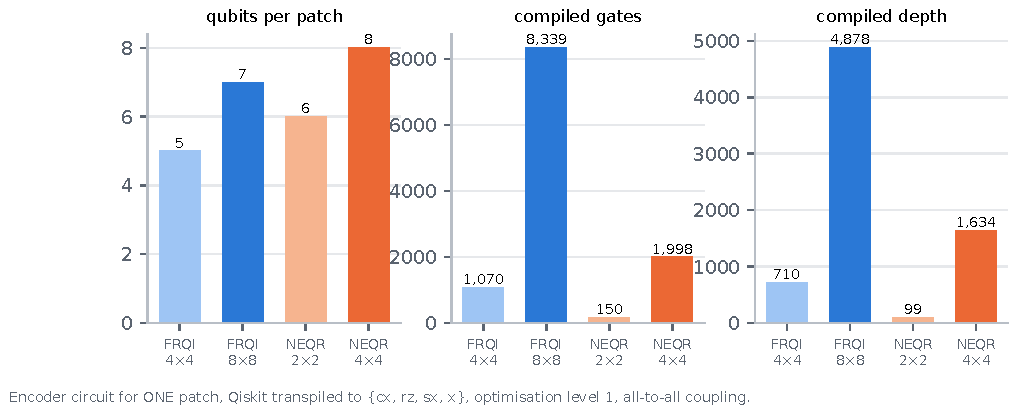
\includegraphics[width=\linewidth]{figures/Fig10_circuit_resources.pdf}
\caption{Qubits, compiled gates and compiled depth of the encoder circuit for one patch.}
\label{fig:fig10}
\end{figure}

\begin{figure}[t]
\centering
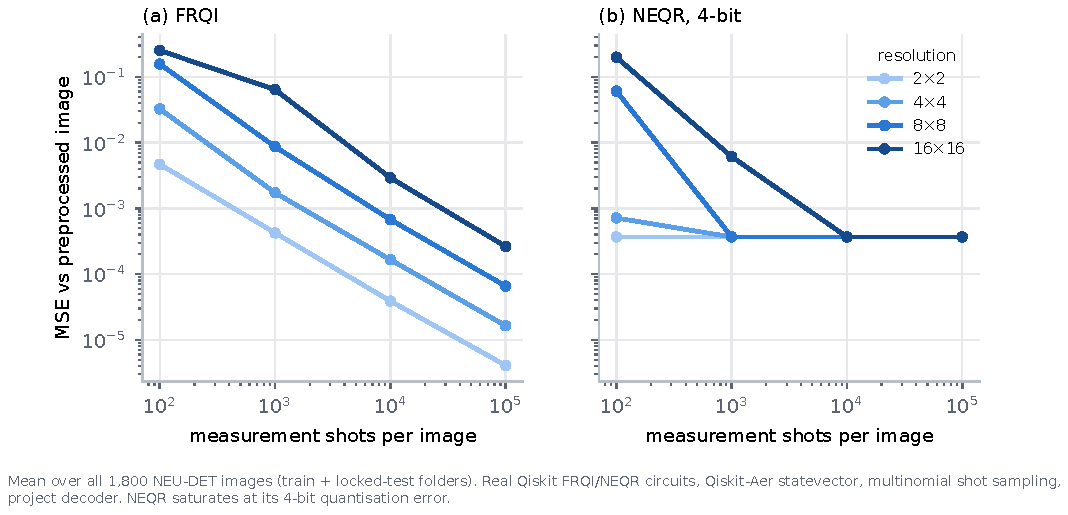
\includegraphics[width=\linewidth]{figures/Fig11_reconstruction_mse_vs_shots.pdf}
\caption{Reconstruction MSE versus measurement shots, mean over all 1,800 images.}
\label{fig:fig11}
\end{figure}

\begin{figure}[t]
\centering
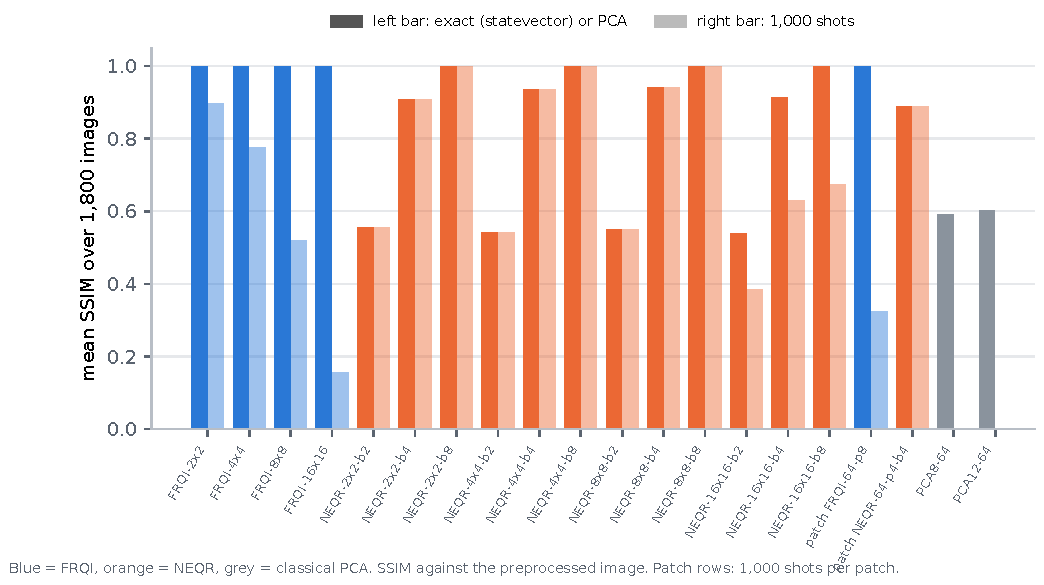
\includegraphics[width=\linewidth]{figures/Fig13_reconstruction_ssim_by_method.pdf}
\caption{Mean SSIM of every reconstruction method (exact and 1,000 shots).}
\label{fig:fig13}
\end{figure}

\begin{figure}[t]
\centering
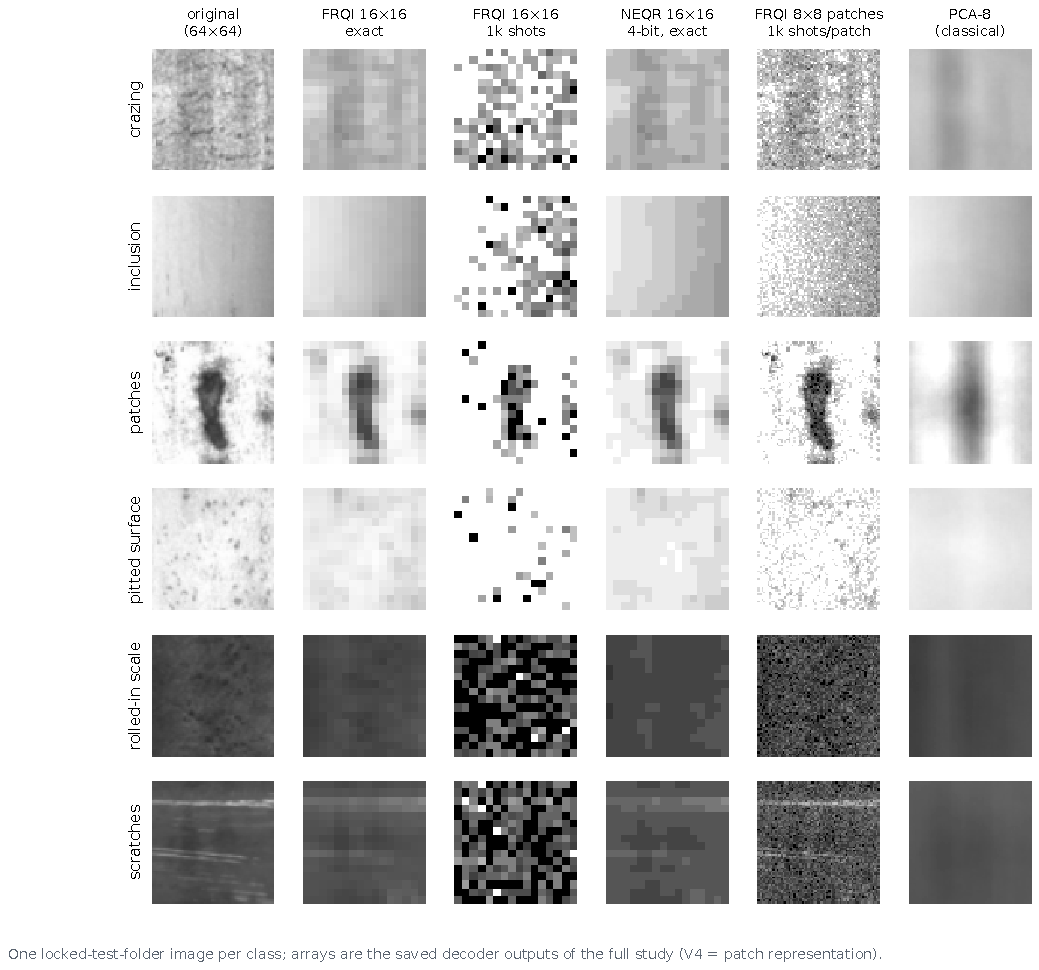
\includegraphics[width=\linewidth]{figures/Fig12_reconstruction_examples.pdf}
\caption{One locked-test-folder image per class reconstructed by representative methods (saved decoder outputs).}
\label{fig:fig12}
\end{figure}

\begin{figure}[t]
\centering
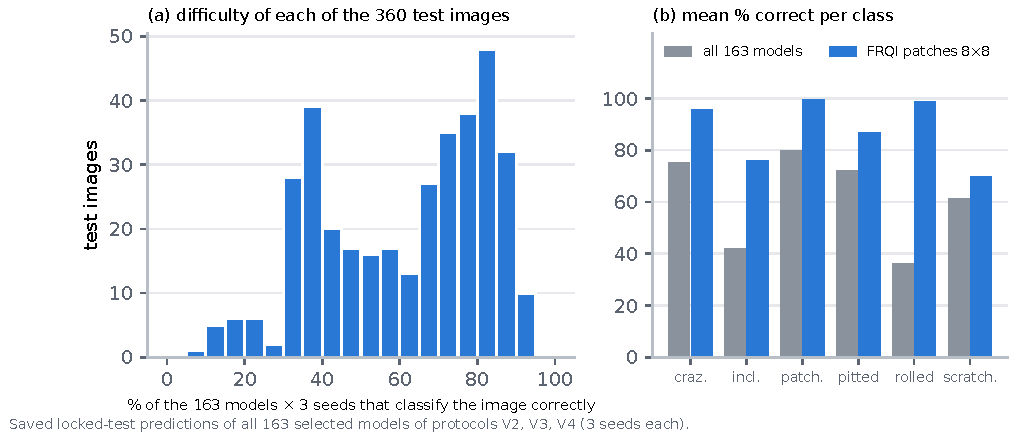
\includegraphics[width=\linewidth]{figures/Fig14_per_image_difficulty.pdf}
\caption{(a) Fraction of all model-seed pairs that classify each test image correctly; (b) mean per class, all models vs V4 FRQI.}
\label{fig:fig14}
\end{figure}

\begin{figure}[t]
\centering
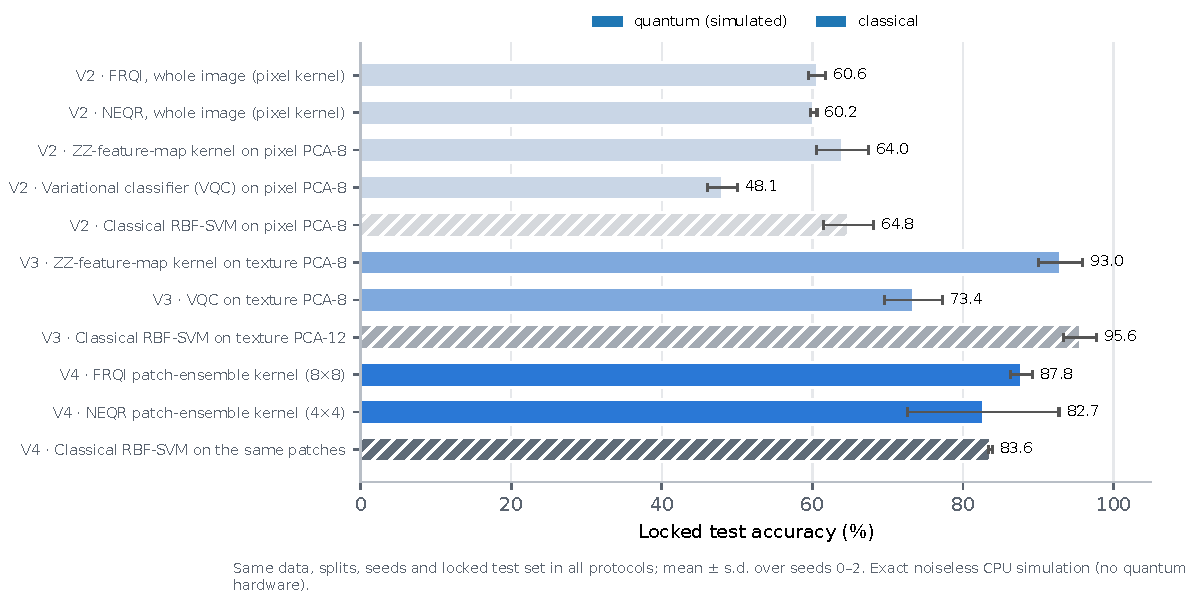
\includegraphics[width=\linewidth]{figures/Fig15_cross_protocol_overview.pdf}
\caption{Key quantum (simulated) and classical models across protocols V2, V3 and V4.}
\label{fig:fig15}
\end{figure}

\begin{table}[t]
\centering
\small
\caption{Table 1. NEU-DET dataset and splits (per class; identical counts for seeds 0, 1, 2)}
\label{tab:tab01}
\resizebox{\linewidth}{!}{%
\begin{tabular}{lllll}
\toprule
Class & Train & Validation & Locked test & Total \\
\midrule
crazing & 180 & 60 & 60 & 300 \\
inclusion & 180 & 60 & 60 & 300 \\
patches & 180 & 60 & 60 & 300 \\
pitted surface & 180 & 60 & 60 & 300 \\
rolled-in scale & 180 & 60 & 60 & 300 \\
scratches & 180 & 60 & 60 & 300 \\
Total & 1080 & 360 & 360 & 1800 \\
\bottomrule
\end{tabular}}
\par\smallskip\footnotesize Train/validation = group-blocked split of the 1,440 NEU-DET train-folder images (group-blocked (blocks of 20 indices), 3 val blocks/class); locked test = the 360 NEU-DET validation-folder images, read once per frozen model.
\end{table}

\begin{table}[t]
\centering
\small
\caption{Table 2. Hyper-parameter grid searched on the validation split (test never used)}
\label{tab:tab02}
\resizebox{\linewidth}{!}{%
\begin{tabular}{lllllll}
\toprule
Group & Image size, patch p, stride s & Encoding option & Normalisation & SVM C & Configs & Runs ($\times$3 seeds) \\
\midrule
FRQI patches 4$\times$4 & 32² p4 s2; 64² p4 s4 & angle $\times$1, 2, 4 & none, stretch & 1, 10, 100, 1000 & 48 & 144 \\
FRQI patches 8$\times$8 & 32² p8 s4; 64² p8 s4; 128² p8 s8 & angle $\times$1, 2, 4 & none, stretch & 1, 10, 100, 1000 & 72 & 216 \\
NEQR patches 2$\times$2 & 32² p2 s1; 64² p2 s2 & 4, 5, 6 bits & none, stretch & 1, 10, 100, 1000 & 48 & 144 \\
NEQR patches 4$\times$4 & 32² p4 s2; 64² p4 s4; 128² p4 s4 & 3, 4 bits & none, stretch & 1, 10, 100, 1000 & 48 & 144 \\
Classical RBF-SVM, same patches & 64² p4 s4; 64² p8 s4; 128² p4 s4 & $\gamma$ 0.3, 1, 3 & none, stretch & 1, 10, 100, 1000 & 72 & 216 \\
Total &  &  &  &  & 288 & 864 \\
\bottomrule
\end{tabular}}
\par\smallskip\footnotesize Selection rule: maximum mean validation macro-F1 over seeds 0–2. Selections were SHA-256 frozen before the locked test was read.
\end{table}

\begin{table}[t]
\centering
\small
\caption{Table 3. Configurations selected by validation macro-F1}
\label{tab:tab03}
\resizebox{\linewidth}{!}{%
\begin{tabular}{lllllllll}
\toprule
Group & Image & Patch / stride & Patches per image & Encoding & Normalisation & C & Qubits per patch state & State dimension D \\
\midrule
FRQI patches 4$\times$4 & 64$\times$64 & 4$\times$4 / 4 & 256 & FRQI, angle $\times$4 & per-image stretch & 1000 & 5 & 32 \\
FRQI patches 8$\times$8 & 64$\times$64 & 8$\times$8 / 4 & 225 & FRQI, angle $\times$4 & per-image stretch & 1000 & 7 & 128 \\
NEQR patches 2$\times$2 & 64$\times$64 & 2$\times$2 / 2 & 1024 & NEQR, 4-bit & none & 1000 & 6 & 64 \\
NEQR patches 4$\times$4 & 128$\times$128 & 4$\times$4 / 4 & 1024 & NEQR, 4-bit & none & 1000 & 8 & 256 \\
Classical RBF-SVM, same patches & 64$\times$64 & 8$\times$8 / 4 & 225 & patch moments, $\gamma$=1 & per-image stretch & 1000 & — (classical) & — \\
\bottomrule
\end{tabular}}
\par\smallskip\footnotesize $\rho$ is a D$\times$D density matrix (average of the patch states). FRQI: 2·log2(p)+1 qubits; NEQR: 2·log2(p)+q qubits.
\end{table}

\begin{table}[t]
\centering
\small
\caption{Table 4. Main results on the locked test set (360 images; mean $\pm$ s.d. over seeds 0–2)}
\label{tab:tab04}
\resizebox{\linewidth}{!}{%
\begin{tabular}{llllll}
\toprule
Model & Type & Validation macro-F1 \% & Test accuracy \% & Test macro-F1 \% & Per-seed test accuracy \% \\
\midrule
FRQI patches 4$\times$4 & quantum (simulated) & 85.7 & 85.3 $\pm$ 1.7 & 85.0 $\pm$ 1.6 & 86.9, 85.3, 83.6 \\
FRQI patches 8$\times$8 & quantum (simulated) & 88.0 & 87.8 $\pm$ 1.5 & 87.5 $\pm$ 1.6 & 86.7, 87.2, 89.4 \\
NEQR patches 2$\times$2 & quantum (simulated) & 88.2 & 81.5 $\pm$ 10.6 & 79.2 $\pm$ 14.1 & 85.6, 69.4, 89.4 \\
NEQR patches 4$\times$4 & quantum (simulated) & 89.2 & 82.7 $\pm$ 10.1 & 80.4 $\pm$ 13.5 & 87.5, 71.1, 89.4 \\
Classical RBF-SVM, same patches & classical & 83.8 & 83.6 $\pm$ 0.3 & 83.3 $\pm$ 0.3 & 83.3, 83.9, 83.6 \\
V2 FRQI, whole image (baseline) & reference & 69.3 & 60.6 $\pm$ 1.2 & 58.3 $\pm$ 1.3 & — \\
V2 NEQR, whole image (baseline) & reference & 72.7 & 60.2 $\pm$ 0.4 & 56.5 $\pm$ 0.4 & — \\
V3 classical texture RBF-SVM (best classical) & reference & 95.3 & 95.6 $\pm$ 2.2 & 95.5 $\pm$ 2.2 & — \\
\bottomrule
\end{tabular}}
\par\smallskip\footnotesize Headline models (pre-declared rule, by validation): FRQI = FRQI patches 8$\times$8, NEQR = NEQR patches 4$\times$4. Exact noiseless CPU simulation (no quantum hardware).
\end{table}

\begin{table}[t]
\centering
\small
\caption{Table 5. The 8 pre-declared paired comparisons (Holm-corrected)}
\label{tab:tab05}
\resizebox{\linewidth}{!}{%
\begin{tabular}{llllllll}
\toprule
Comparison (a vs b) & Acc. a \% & Acc. b \% & $\Delta$ pp & 95\% CI pp & p (Holm) & Significant & McNemar a-only:b-only (seeds 0/1/2) \\
\midrule
V4 FRQI vs V2 FRQI (E1b-frqi8-qkc-scaled) & 87.8 & 60.6 & +27.1 & [+21.7, +32.7] & $<$0.001 & yes & 114:25 / 118:21 / 123:16 \\
V4 FRQI vs V3 FRQI (V3-frqi8) & 87.8 & 57.5 & +30.3 & [+25.1, +35.4] & $<$0.001 & yes & 120:22 / 134:19 / 131:17 \\
V4 NEQR vs V2 NEQR (E2-neqr16-b4-qkc) & 82.7 & 60.2 & +22.5 & [+18.5, +26.7] & $<$0.001 & yes & 108:11 / 48:7 / 119:14 \\
V4 FRQI vs V4 NEQR & 87.8 & 82.7 & +5.1 & [+1.1, +9.0] & 0.045 & yes & 30:33 / 87:29 / 32:32 \\
V4 FRQI vs classical patch-moment RBF-SVM & 87.8 & 83.6 & +4.2 & [+0.5, +7.7] & 0.060 & no & 36:24 / 34:22 / 42:21 \\
V4 NEQR vs classical patch-moment RBF-SVM & 82.7 & 83.6 & -0.9 & [-4.9, +3.1] & 0.678 & no & 40:25 / 34:80 / 44:23 \\
V4 FRQI vs classical texture RBF-SVM (V3-tex12c-rbfsvm) & 87.8 & 95.6 & -7.8 & [-10.9, -4.7] & $<$0.001 & yes & 12:40 / 11:36 / 6:37 \\
V4 NEQR vs classical texture RBF-SVM (V3-tex12c-rbfsvm) & 82.7 & 95.6 & -12.9 & [-15.8, -10.0] & $<$0.001 & yes & 7:32 / 3:86 / 5:36 \\
\bottomrule
\end{tabular}}
\par\smallskip\footnotesize Paired sign-flip permutation test (10,000) on per-image correctness averaged over seeds; bootstrap 95\% CI; Holm correction over 8 tests.
\end{table}

\begin{table}[t]
\centering
\small
\caption{Table 6. Per-class F1 \% on the locked test set (mean over seeds 0–2)}
\label{tab:tab06}
\resizebox{\linewidth}{!}{%
\begin{tabular}{lllllll}
\toprule
Model & crazing & inclusion & patches & pitted surface & rolled-in scale & scratches \\
\midrule
FRQI patches 4$\times$4 & 85.8 & 85.5 & 94.8 & 74.7 & 89.8 & 79.6 \\
FRQI patches 8$\times$8 & 93.1 & 84.0 & 95.8 & 81.5 & 89.5 & 81.3 \\
NEQR patches 2$\times$2 & 88.6 & 72.7 & 91.6 & 82.8 & 62.1 & 77.3 \\
NEQR patches 4$\times$4 & 89.5 & 72.7 & 91.4 & 80.0 & 65.0 & 84.0 \\
Classical RBF-SVM, same patches & 83.5 & 67.8 & 92.9 & 66.7 & 93.0 & 95.9 \\
\bottomrule
\end{tabular}}
\end{table}

\begin{table}[t]
\centering
\small
\caption{Table 7. Encoder circuit resources for ONE patch state (Qiskit, transpiled)}
\label{tab:tab07}
\resizebox{\linewidth}{!}{%
\begin{tabular}{llllllll}
\toprule
Group & Qubits & Logical gates & Logical depth & Compiled gates & Compiled depth & CX (compiled) & Patches per image \\
\midrule
FRQI patches 4$\times$4 & 5 & 1093 & 705 & 1070 & 710 & 384 & 256 \\
FRQI patches 8$\times$8 & 7 & 8583 & 4875 & 8339 & 4878 & 3584 & 225 \\
NEQR patches 2$\times$2 & 6 & 20 & 15 & 150 & 99 & 55 & 1024 \\
NEQR patches 4$\times$4 & 8 & 106 & 65 & 1998 & 1634 & 694 & 1024 \\
\bottomrule
\end{tabular}}
\par\smallskip\footnotesize Basis {cx, rz, sx, x}, optimisation level 1, all-to-all coupling. A swap test between two patch states uses 2·qubits + 1 qubits.
\end{table}

\begin{table}[t]
\centering
\small
\caption{Table 8. Reconstruction of all 1,800 NEU-DET images by every method (mean MSE / SSIM)}
\label{tab:tab08}
\resizebox{\linewidth}{!}{%
\begin{tabular}{llllllll}
\toprule
Method & Encoding & Qubits & MSE exact (statevector) & MSE 1,000 shots & MSE most shots & SSIM 1,000 shots & Images exact (of 1,800) \\
\midrule
R-FRQI-2x2 & FRQI & 3 & 0 (exact) & 4.24e-04 & 4.09e-06 (100,000) & 0.897 & 1,800 \\
R-FRQI-4x4 & FRQI & 5 & 0 (exact) & 1.73e-03 & 1.64e-05 (100,000) & 0.775 & 1,800 \\
R-FRQI-8x8 & FRQI & 7 & 0 (exact) & 8.66e-03 & 6.57e-05 (100,000) & 0.518 & 1,800 \\
R-FRQI-16x16 & FRQI & 9 & 0 (exact) & 6.40e-02 & 2.64e-04 (100,000) & 0.156 & 1,800 \\
R-NEQR-2x2-b2 & NEQR & 4 & 9.01e-03 & 9.01e-03 & 9.01e-03 (100,000) & 0.554 & 0 \\
R-NEQR-2x2-b4 & NEQR & 6 & 3.68e-04 & 3.68e-04 & 3.68e-04 (100,000) & 0.907 & 0 \\
R-NEQR-2x2-b8 & NEQR & 10 & 0 (exact) & 0 (exact) & 0 (exact) (100,000) & 1.000 & 1,800 \\
R-NEQR-4x4-b2 & NEQR & 6 & 8.97e-03 & 8.97e-03 & 8.97e-03 (100,000) & 0.542 & 0 \\
R-NEQR-4x4-b4 & NEQR & 8 & 3.68e-04 & 3.68e-04 & 3.68e-04 (100,000) & 0.934 & 0 \\
R-NEQR-4x4-b8 & NEQR & 12 & 0 (exact) & 0 (exact) & 0 (exact) (100,000) & 1.000 & 1,800 \\
R-NEQR-8x8-b2 & NEQR & 8 & 8.94e-03 & 8.94e-03 & 8.94e-03 (100,000) & 0.549 & 0 \\
R-NEQR-8x8-b4 & NEQR & 10 & 3.69e-04 & 3.69e-04 & 3.69e-04 (100,000) & 0.941 & 0 \\
R-NEQR-8x8-b8 & NEQR & 14 & 0 (exact) & 0 (exact) & 0 (exact) (100,000) & 1.000 & 1,800 \\
R-NEQR-16x16-b2 & NEQR & 10 & 8.93e-03 & 1.48e-02 & 8.93e-03 (100,000) & 0.385 & 0 \\
R-NEQR-16x16-b4 & NEQR & 12 & 3.68e-04 & 6.12e-03 & 3.68e-04 (100,000) & 0.630 & 0 \\
R-NEQR-16x16-b8 & NEQR & 16 & 0 (exact) & 5.75e-03 & 0 (exact) (100,000) & 0.673 & 1,800 \\
P-FRQI-64-p8 & FRQI & 7 & 0 (exact) & 8.67e-03 & 6.70e-04 (10,000) & 0.323 & 1,800 \\
P-NEQR-64-p4-b4 & NEQR & 8 & 3.67e-04 & 3.67e-04 & 3.67e-04 (10,000) & 0.888 & 0 \\
C-PCA8-64 & classical PCA & — & 4.66e-03 & — & — & 0.590 & — \\
C-PCA12-64 & classical PCA & — & 3.85e-03 & — & — & 0.603 & — \\
\bottomrule
\end{tabular}}
\par\smallskip\footnotesize R- = whole image r$\times$r; NEQR -bN = N-bit intensity; P- = V4 patch representation (shots per patch); C- = classical PCA (fit on seed-0 train). Real Qiskit circuits + Aer statevector + multinomial shots.
\end{table}

\begin{table}[t]
\centering
\small
\caption{Table 9. Key models across protocols V2 $\rightarrow$ V3 $\rightarrow$ V4 (locked test accuracy \%)}
\label{tab:tab09}
\resizebox{\linewidth}{!}{%
\begin{tabular}{llll}
\toprule
Protocol & Model & Type & Test accuracy \% \\
\midrule
V2 & FRQI, whole image (pixel kernel) & quantum & 60.6 $\pm$ 1.2 \\
V2 & NEQR, whole image (pixel kernel) & quantum & 60.2 $\pm$ 0.4 \\
V2 & ZZ-feature-map kernel on pixel PCA-8 & quantum & 64.0 $\pm$ 3.5 \\
V2 & Variational classifier (VQC) on pixel PCA-8 & quantum & 48.1 $\pm$ 1.9 \\
V2 & Classical RBF-SVM on pixel PCA-8 & classical & 64.8 $\pm$ 3.3 \\
V3 & ZZ-feature-map kernel on texture PCA-8 & quantum & 93.0 $\pm$ 3.0 \\
V3 & VQC on texture PCA-8 & quantum & 73.4 $\pm$ 3.8 \\
V3 & Classical RBF-SVM on texture PCA-12 & classical & 95.6 $\pm$ 2.2 \\
V4 & FRQI patch-ensemble kernel (8$\times$8) & quantum & 87.8 $\pm$ 1.5 \\
V4 & NEQR patch-ensemble kernel (4$\times$4) & quantum & 82.7 $\pm$ 10.1 \\
V4 & Classical RBF-SVM on the same patches & classical & 83.6 $\pm$ 0.3 \\
\bottomrule
\end{tabular}}
\par\smallskip\footnotesize Same dataset, splits, seeds and locked test set in every protocol. Quantum = exact CPU simulation.
\end{table}

\begin{table}[t]
\centering
\small
\caption{Table 10. Automated integrity checks (17/17 pass)}
\label{tab:tab10}
\resizebox{\linewidth}{!}{%
\begin{tabular}{ll}
\toprule
Check & Result \\
\midrule
historical V0 results: 0 changed, 0 missing & PASS \\
V2 manifest/splits/caches unchanged (SHA-256, in qml\_v2 and qml\_v3) & PASS \\
V4 copies of manifest/splits/image caches identical to the V3/V2 originals & PASS \\
no Protocol V2 result file modified or added since V3 was finalised & PASS \\
no Protocol V3 result file modified or added since V3 was finalised & PASS \\
all 70 V3 selection files unchanged since the V3 freeze & PASS \\
V4 selection files unchanged since the V4 freeze & PASS \\
every V4 locked-test access after the freeze, one per frozen group & PASS \\
test predictions exist only for the frozen configurations & PASS \\
no selection file contains a test metric & PASS \\
864 candidate runs, 0 failed & PASS \\
test accuracy recomputed from predictions.csv (360 locked images per run) & PASS \\
FRQI headline chosen by validation & PASS \\
NEQR headline chosen by validation & PASS \\
comparisons are exactly the 8 pre-declared ones & PASS \\
every V4 quantum group records a real FRQI/NEQR encoder circuit (Qiskit, transpiled) & PASS \\
classical control has no circuit and is labelled classical & PASS \\
\bottomrule
\end{tabular}}
\end{table}

